% 第4章第4节：高斯过程（均值与协方差、半正定性、样本路径与核空间）。

\section{高斯过程}
\label{sec:spp-gaussian-processes}

Kolmogorov扩张定理把构造过程归结为写下一族相容的有限维分布。高斯分布是最容易写全的一族：只要给出均值和协方差，任意有限个位置上的联合分布就确定了，并且删去坐标后的边缘仍是高斯分布。本节利用这一点，在任意索引集上构造随机函数，索引可以是时间，也可以是空间位置或一般输入。我们先说明均值函数与协方差函数怎样确定过程、协方差需要满足什么条件，再讨论样本路径的正则性，并把协方差作为随机函数的规律与它作为再生核所定义的确定性函数空间区分开来。由观测推断未知函数的高斯过程回归不在本节讨论。

\subsection{均值、协方差与联合高斯规律}
\label{sec:spp-gp-definition}

\paragraph{允许奇异协方差的高斯向量}
有限维高斯分布通常用密度定义，这要求协方差矩阵正定。构造过程时却经常遇到奇异的协方差：例如三个位置上的读数可能由两个随机系数完全决定。下面采用不依赖密度的说法。随机向量$\bm Y\in\mathbb R^m$称为高斯向量，若存在$\bm\mu\in\mathbb R^m$、矩阵$\bm A\in\mathbb R^{m\times r}$和由独立标准高斯变量组成的$\bm Z\in\mathbb R^r$，使$\bm Y=\bm\mu+\bm A\bm Z$。此时$\mathbb E\bm Y=\bm\mu$，$\operatorname{Cov}(\bm Y)=\bm A\bm A^\top$。

这个定义有三条性质需要用到。第一，任意对称半正定矩阵$\bm\Sigma$都可以作为协方差：取谱分解$\bm\Sigma=\bm Q\bm\Lambda\bm Q^\top$，令$\bm A=\bm Q\bm\Lambda^{1/2}$即可。第二，分布只依赖$(\bm\mu,\bm\Sigma)$：$\bm Y$的特征函数为$\mathbb E e^{\mathrm i\bm c^\top\bm Y}=\exp(\mathrm i\bm c^\top\bm\mu-\tfrac12\bm c^\top\bm\Sigma\bm c)$，而特征函数决定分布；记作$\bm Y\sim\mathcal N(\bm\mu,\bm\Sigma)$。第三，线性像仍是高斯向量：对矩阵$\bm B$，$\bm B\bm Y=\bm B\bm\mu+(\bm B\bm A)\bm Z$，所以$\bm B\bm Y\sim\mathcal N(\bm B\bm\mu,\bm B\bm\Sigma\bm B^\top)$。$\bm\Sigma$正定时，这与用密度定义的\term{多元高斯分布}（multivariate Gaussian distribution）一致，后者及其仿射变换性质可参考\BookChapterRef{chap:random-vectors}{卷一“随机向量与联合分布”章}；$\bm\Sigma$奇异时，$\bm Y$集中在一个仿射子空间上，没有密度。

\paragraph{高斯过程的定义}
把“任意有限个读数联合高斯”作为定义，就得到高斯过程。

\begin{definition}[高斯过程]
\label{def:spp-gaussian-process}
实值随机过程$F=(F(x))_{x\in\mathcal X}$称为\term{高斯过程}（Gaussian process），若对任意正整数$m$和任意$x_1,\ldots,x_m\in\mathcal X$，随机向量$(F(x_1),\ldots,F(x_m))^\top$都是高斯向量。函数
\[
  m(x)=\mathbb EF(x),\qquad k(x,x')=\operatorname{Cov}\bigl(F(x),F(x')\bigr)
\]
分别称为它的\term{均值函数}（mean function）与\term{协方差函数}（covariance function），记作$F\sim\mathcal{GP}(m,k)$。
\end{definition}

索引集$\mathcal X$可以是任意集合，不需要顺序，也不需要拓扑。由第三条性质，$(F(x_1),\ldots,F(x_m))^\top$的分布是均值为$(m(x_i))_i$、协方差为$(k(x_i,x_j))_{i,j}$的高斯分布，所以$m$与$k$决定了全部有限维分布，从而决定了路径规律。

定义中“联合”二字不可省略。设$X\sim\mathcal N(0,1)$，符号$S$与$X$独立、等概率取$\pm1$。则$X$与$SX$都服从$\mathcal N(0,1)$，且$\operatorname{Cov}(X,SX)=\mathbb ES\cdot\mathbb EX^2=0$。但$X+SX$以概率$1/2$恰好为$0$，以概率$1/2$等于$2X$，它不是高斯变量；所以$(X,SX)$不是高斯向量，尽管两个坐标各自高斯且不相关。逐点高斯并不足以构成高斯过程。

\paragraph{存在性：半正定是充要条件}
哪些函数$k$可以作为协方差函数？答案是半正定性，它既是必要的，也是充分的。

\begin{theorem}[高斯过程的存在与唯一]
\label{thm:spp-gp-existence}
设$\mathcal X$是非空集合，$m:\mathcal X\to\mathbb R$，$k:\mathcal X\times\mathcal X\to\mathbb R$。存在以$m$为均值函数、$k$为协方差函数的高斯过程，当且仅当$k$对称，并且对任意有限个$x_1,\ldots,x_n\in\mathcal X$和实数$c_1,\ldots,c_n$都有
\begin{equation}
  \sum_{i,j=1}^nc_ic_j\,k(x_i,x_j)\ge0 .
  \label{eq:spp-psd}
\end{equation}
满足这一条件时，过程在$(\mathbb R^{\mathcal X},\mathcal B(\mathbb R)^{\otimes\mathcal X})$上的路径规律唯一。
\end{theorem}

\begin{proof}
必要性：若过程存在，协方差由
\[
  \operatorname{Cov}(F(x),F(x'))=\operatorname{Cov}(F(x'),F(x))
\]
对称，并且$\sum_{i,j}c_ic_jk(x_i,x_j)=\operatorname{Var}\bigl(\sum_ic_iF(x_i)\bigr)\ge0$。这一步只用到二阶矩，所以任何二阶矩有限的过程的协方差函数都满足式~\eqref{eq:spp-psd}。

充分性：对有限集$J\subseteq\mathcal X$，矩阵$\bm K_J=(k(s,t))_{s,t\in J}$对称且由式~\eqref{eq:spp-psd}半正定，令$\mu_J=\mathcal N\bigl((m(t))_{t\in J},\bm K_J\bigr)$。对有限集$J\subseteq K$，限制映射$\pi_{K,J}$是删去坐标的线性映射，由线性像的性质，$\mu_K\circ\pi_{K,J}^{-1}$是均值为$(m(t))_{t\in J}$、协方差为$\bm K_K$的子矩阵$\bm K_J$的高斯分布，即$\mu_J$。所以这一族相容。$\mathbb R$是标准Borel空间，由定理~\ref{thm:spp-kolmogorov-extension}得到所需过程。唯一性来自有限维分布由$(m,k)$决定以及定理~\ref{thm:spp-path-law}。
\end{proof}

满足式~\eqref{eq:spp-psd}的对称函数称为\term{半正定}（positive semidefinite）核。定理把“构造一个高斯过程”化为“检查一个二元函数半正定”，后者是纯粹的确定性问题。

\paragraph{几种协方差结构}
下面几类协方差依次说明，核怎样规定读数之间的依赖，以及怎样检查半正定性。

\emph{常数核。}$k(x,x')\equiv\sigma^2$。取$Z\sim\mathcal N(0,1)$，令$F(x)=\sigma Z$对一切$x$成立，即得此过程：所有位置读数相同，整条路径是一条随机高度的水平线。任意$n$个位置的协方差矩阵秩为$1$。

\emph{有限随机基展开。}取确定函数$\varphi_1,\ldots,\varphi_r$和独立标准高斯变量$Z_1,\ldots,Z_r$，令$F(x)=\sum_{j=1}^rZ_j\varphi_j(x)$。则$k(x,x')=\sum_j\varphi_j(x)\varphi_j(x')$，半正定性自动成立：$\sum_{i,l}c_ic_lk(x_i,x_l)=\sum_j\bigl(\sum_ic_i\varphi_j(x_i)\bigr)^2\ge0$。任意多个位置上的读数都由$r$个系数决定，协方差矩阵的秩至多为$r$。例如$F(x)=A+Bx$，$A,B$独立标准高斯，$k(x,x')=1+xx'$；在$x=0,1,2$处
\[
  \bm K=\begin{pmatrix}1&1&1\\1&2&3\\1&3&5\end{pmatrix},\qquad \det\bm K=0,
\]
因为三个读数满足$F(0)-2F(1)+F(2)=0$。

\emph{平稳核。}在$\mathcal X=\mathbb R$上，若$k(x,x')=\kappa(x-x')$只依赖位置差，则读数的依赖不随整体平移改变。常用的有\term{平方指数核}（squared exponential kernel）$\kappa(h)=\sigma^2e^{-h^2/(2\ell^2)}$和\term{指数核}（exponential kernel）$\kappa(h)=\sigma^2e^{-|h|/\ell}$，长度尺度$\ell$控制相关性衰减的距离。检查它们半正定有一个统一的办法：若$\kappa(h)=\sigma^2\,\mathbb Ee^{\mathrm iWh}$是某个对称分布$W$的特征函数乘以$\sigma^2$，则
\[
  \sum_{i,j}c_ic_j\kappa(x_i-x_j)=\sigma^2\,\mathbb E\Bigl|\sum_jc_je^{\mathrm iWx_j}\Bigr|^2\ge0 .
\]
$e^{-h^2/(2\ell^2)}$是$\mathcal N(0,\ell^{-2})$的特征函数，$e^{-|h|/\ell}$是密度为$\ell/\bigl(\pi(1+\ell^2w^2)\bigr)$的Cauchy分布的特征函数，所以两者都半正定。\term{周期核}（periodic kernel）$k(x,x')=\sigma^2\exp\bigl(-2\sin^2(\pi(x-x')/p)/\ell^2\bigr)$可以化归为平方指数核：令$\bm u(x)=(\cos(2\pi x/p),\sin(2\pi x/p))$，则$|\bm u(x)-\bm u(x')|^2=4\sin^2(\pi(x-x')/p)$，周期核就是平面$\mathbb R^2$上的平方指数核在点$\bm u(x_1),\ldots,\bm u(x_n)$处的取值。平方指数核在$\mathbb R^2$上的半正定性同样来自二元高斯分布的特征函数。

\emph{Brownian核。}在$\mathcal X=[0,\infty)$上，$k(s,t)=\min(s,t)$也称\term{最小值核}（minimum kernel）。它半正定，因为
\[
  \sum_{i,j}c_ic_j\min(t_i,t_j)=\int_0^\infty\Bigl(\sum_ic_i\mathbb I_{\{u\le t_i\}}\Bigr)^2\mathrm du\ge0 ,
\]
这里用了$\int_0^\infty\mathbb I_{\{u\le t_i\}}\mathbb I_{\{u\le t_j\}}\,\mathrm du=\min(t_i,t_j)$。均值为零、协方差为$\min(s,t)$的高斯过程就是Brownian运动的有限维规律：对$s<t$，$\operatorname{Var}(F(t)-F(s))=t-2s+s=t-s$，不相交区间上的增量不相关因而独立。

并非每个看起来合理的“相似度”都半正定。取$k(x,x')=\mathbb I_{\{|x-x'|\le1\}}$，即距离不超过$1$的两点完全相关、否则不相关。在$x=0,0.75,1.5$处，系数$c=(1,-1,1)$给出
\[
  \sum_{i,j}c_ic_jk(x_i,x_j)=3-2\cdot1-2\cdot1+2\cdot0=-1<0 ,
\]
所以不存在以它为协方差的过程。

图~\ref{fig:spp-gp-kernels}把四个核的协方差矩阵画成热图，并在每个核下抽取三条样本路径。对角线附近的颜色宽度对应相关距离：平方指数核的路径光滑，指数核的路径粗糙，周期核的路径以$p=0.5$为周期重复，Brownian核的路径从$0$出发、方差随$t$增长。前三个核在每个位置的方差都是$1$，路径外观的差别完全来自位置之间的相关结构；Brownian核的方差$t$则随位置增长。

\begin{figure*}[htbp]
  \centering
  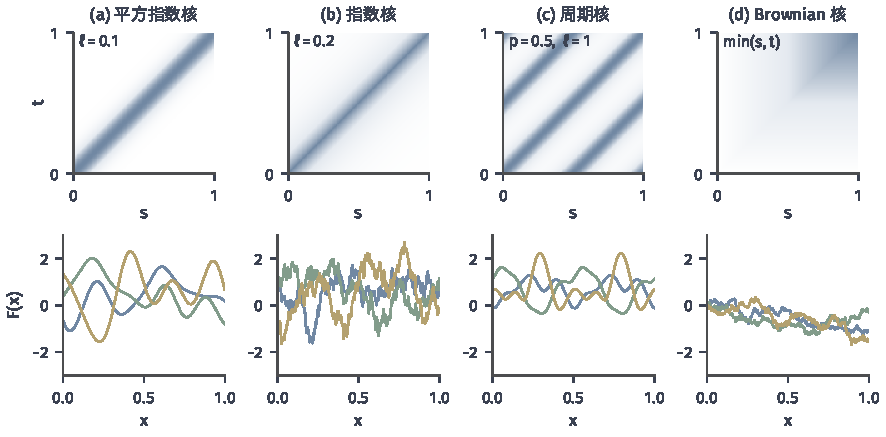
\includegraphics[width=150mm]{figures/03-optimization-evolution-and-signals/02-processes-and-trajectory-evolution/matplotlib/spp-gp-kernels/figure.pdf}
  \caption{四种协方差函数及相应高斯过程的样本路径，定义域$[0,1]$，$\sigma^2=1$。上排为$k(s,t)$在$301\times301$网格上的热图（白色为$0$，蓝色为$1$）；下排为对应的三条样本路径，用网格协方差矩阵的特征分解抽样（固定随机种子，三条路径在四个核下使用同一组标准高斯向量）。(a)平方指数核，$\ell=0.1$；(b)指数核，$\ell=0.2$；(c)周期核，$p=0.5$，$\ell=1$；(d)Brownian核$\min(s,t)$。}
  \label{fig:spp-gp-kernels}
\end{figure*}

索引不必是一维时间。在平面区域上取$k(\bm x,\bm x')=\sigma^2e^{-|\bm x-\bm x'|^2/(2\ell^2)}$，得到的随机场在距离小于$\ell$的位置上读数相近，可用来描述一片区域上的气温偏差；这里没有“过去”和“将来”，逐步构造无从谈起，扩张定理却照样适用。

\paragraph{在有限网格上抽样}
计算机只能在有限个位置上抽样。给定网格$x_1,\ldots,x_n$，计算矩阵$\bm K=(k(x_i,x_j))_{i,j}$，求一个分解$\bm K=\bm A\bm A^\top$，再令$(F(x_i))_i=(m(x_i))_i+\bm A\bm Z$，其中$\bm Z$是$n$维标准高斯向量。$\bm K$正定时常用Cholesky分解，计算量为$O(n^3)$，存储为$O(n^2)$；$\bm K$奇异或接近奇异时（例如平方指数核在密集网格上），可以用特征分解并把舍入误差造成的微小负特征值截为零，图~\ref{fig:spp-gp-kernels}就是这样生成的。实践中也常在对角线上加一个小量$\epsilon$再做Cholesky分解；这相当于给每个读数加上独立的$\mathcal N(0,\epsilon)$噪声，抽到的是略有不同的过程，$\epsilon$应当相对于核的尺度足够小。

\paragraph{有限基展开逼近Brownian运动}
有限随机基展开不仅是一个例子，也是构造一般高斯过程的方法。对Brownian核，令$a_k=(k-\tfrac12)\pi$，$e_k(t)=\sqrt2\sin(a_kt)/a_k$，$k\ge1$。对$s,t\in[0,1]$有恒等式
\begin{equation}
  \min(s,t)=\sum_{k=1}^\infty e_k(s)e_k(t) .
  \label{eq:spp-min-expansion}
\end{equation}
验证如下：$\{\sqrt2\sin(a_kt)\}_{k\ge1}$是$L^2[0,1]$的标准正交基；固定$s$，函数$t\mapsto\min(s,t)$在这组基下的系数为
\[
  \begin{aligned}
  \sqrt2\int_0^1\min(s,t)\sin(a_kt)\,\mathrm dt
  &=\sqrt2\Bigl(\int_0^st\sin(a_kt)\,\mathrm dt+s\int_s^1\sin(a_kt)\,\mathrm dt\Bigr)\\
  &=\frac{\sqrt2\sin(a_ks)}{a_k^2},
  \end{aligned}
\]
其中分部积分后用了$\cos a_k=0$。于是$\min(s,\cdot)=\sum_k\frac{\sqrt2\sin(a_ks)}{a_k^2}\sqrt2\sin(a_k\cdot)$在$L^2$意义下成立；右边的级数被$\sum_k2/a_k^2<\infty$一致控制，因而绝对一致收敛到一个连续函数，它与连续函数$\min(s,\cdot)$几乎处处相等，故处处相等。

取独立标准高斯变量$Z_1,Z_2,\ldots$，令$W^{(m)}(t)=\sum_{k=1}^mZ_ke_k(t)$。每个$W^{(m)}$是有限基展开的高斯过程，协方差为式~\eqref{eq:spp-min-expansion}的前$m$项部分和。对固定的$t$，各项独立、均值为零，方差之和$\sum_ke_k(t)^2=t$有限，所以级数几乎必然且在$L^2$中收敛；极限$W(t)$是高斯变量，协方差由式~\eqref{eq:spp-min-expansion}给出$\min(s,t)$。图~\ref{fig:spp-kl-expansion}用同一组系数画出$m=1,4,16,1024$时的部分和：项数少时路径光滑，每加入一组高频项就添上更细的起伏，逐渐接近Brownian路径的粗糙外形。这类按协方差的特征函数展开的表示称为\term{Karhunen--Loève展开}（Karhunen--Loève expansion）。

\begin{figure}[htbp]
  \centering
  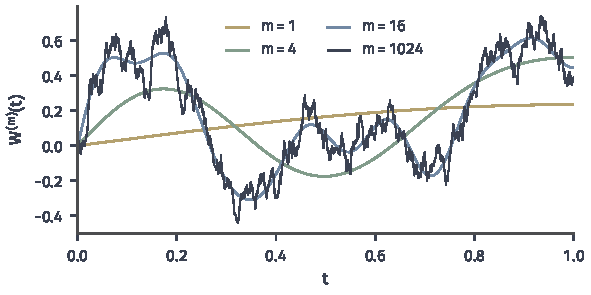
\includegraphics[width=100mm]{figures/03-optimization-evolution-and-signals/02-processes-and-trajectory-evolution/matplotlib/spp-kl-expansion/figure.pdf}
  \caption{Brownian运动的有限基展开$W^{(m)}(t)=\sum_{k\le m}Z_k\sqrt2\sin\bigl((k-\tfrac12)\pi t\bigr)/\bigl((k-\tfrac12)\pi\bigr)$。四条曲线使用同一组独立标准高斯系数$Z_1,Z_2,\ldots$（固定随机种子），仅截断项数$m=1,4,16,1024$不同。每条部分和都是光滑函数，随项数增加逐步出现更细的起伏。}
  \label{fig:spp-kl-expansion}
\end{figure}

\subsection{样本路径与核空间的区别}
\label{sec:spp-gp-paths-rkhs}

\paragraph{增量方差控制路径}
高斯过程的路径性质由协方差决定，具体地说由增量方差决定。设$F\sim\mathcal{GP}(0,k)$，令
\[
  d^2(s,t)=\mathbb E\bigl(F(t)-F(s)\bigr)^2=k(t,t)-2k(s,t)+k(s,s).
\]
增量$F(t)-F(s)\sim\mathcal N(0,d^2(s,t))$，它的高阶矩完全由$d$决定：$\mathbb E|F(t)-F(s)|^{2r}=(2r-1)!!\,d(s,t)^{2r}$。于是只要$d^2$随间隔以幂次衰减，就可以选足够高的矩阶使用Kolmogorov连续性准则。

\begin{theorem}[高斯过程的连续版本]
\label{thm:spp-gp-continuity}
设$F\sim\mathcal{GP}(0,k)$，索引集为$[0,1]$。若存在$C<\infty$与$\alpha>0$使
\[
  d^2(s,t)\le C|t-s|^\alpha,\qquad s,t\in[0,1],
\]
则$F$有连续版本，并且对每个$\gamma\in(0,\alpha/2)$，其几乎所有路径都是$\gamma$阶Hölder连续的。
\end{theorem}

\begin{proof}
取正整数$r$使$r\alpha>1$。则$\mathbb E|F(t)-F(s)|^{2r}\le(2r-1)!!\,C^r|t-s|^{r\alpha}$，满足定理~\ref{thm:spp-kolmogorov-continuity}的条件，其中$p=2r$，$\beta=r\alpha-1$。所得Hölder指数可以取任意小于$\beta/p=\alpha/2-1/(2r)$的值；$r$可以任意大，于是对任意$\gamma<\alpha/2$都成立。
\end{proof}

对Brownian核，$d^2(s,t)=|t-s|$，$\alpha=1$，路径是任意$\gamma<1/2$阶Hölder连续的，这与第~\ref{sec:spp-versions}小节的直接计算一致。对指数核，$d^2(s,t)=2\sigma^2(1-e^{-|t-s|/\ell})\le2\sigma^2|t-s|/\ell$，同样$\alpha=1$：它的路径与Brownian路径一样粗糙，这正是图~\ref{fig:spp-gp-kernels}(b)中看到的。对平方指数核，$1-e^{-u}\le u$给出$d^2(s,t)\le\sigma^2|t-s|^2/\ell^2$，$\alpha=2$，定理给出任意$\gamma<1$阶Hölder连续；它的路径实际上更光滑（任意阶可微），这需要对导数过程再做类似的估计，此处不展开。

\paragraph{均方连续不等于路径连续}
若$d(s,t)\to0$（$s\to t$），称过程\term{均方连续}（mean-square continuous）。这只说明每个固定时刻附近的增量在平均意义上很小，并不控制所有时刻同时发生的事。速率$\lambda$的Poisson计数过程是一个非高斯的例子：$\mathbb E(N_t-N_s)^2=\lambda h+\lambda^2h^2\to0$，它均方连续，而几乎每条路径都有跳跃。对高斯过程，均方连续同样不足以保证连续版本：增量标准差趋于零的速度若太慢，例如只像$(\log(1/h))^{-1/2}$那样衰减，可以构造出在每个区间上几乎必然无界的平稳高斯过程。关于高斯过程路径连续的精确判据涉及度量熵，本书不展开；定理~\ref{thm:spp-gp-continuity}的幂次条件是实践中最常用的充分条件。

\paragraph{同一个核的两种用途}
半正定核在函数空间部分以另一种身份出现过：每个半正定核$k$唯一确定一个由$\mathcal X$上函数组成的Hilbert空间$H_k$，称为\term{再生核Hilbert空间}（reproducing kernel Hilbert space），其中$k(\cdot,x)\in H_k$，并且对每个$f\in H_k$有再生性质$\langle f,k(\cdot,x)\rangle_{H_k}=f(x)$；可参考\BookChapterRef{chap:rkhs}{卷二“再生核Hilbert空间”章}。于是同一个$k$有两种用途：作为协方差，它规定一个随机函数的规律；作为再生核，它规定一个确定性的函数空间及其范数。两者很容易被混为一谈，以为高斯过程的样本就是$H_k$中的随机元素。

有限维情形下这样想是对的。设$F=\sum_{j=1}^rZ_j\varphi_j$，$\varphi_1,\ldots,\varphi_r$线性无关，则$k=\sum_j\varphi_j\otimes\varphi_j$，$H_k$就是$\operatorname{span}\{\varphi_1,\ldots,\varphi_r\}$，并且$\bigl\|\sum_ja_j\varphi_j\bigr\|_{H_k}^2=\sum_ja_j^2$。每个样本$F$都落在$H_k$中，范数平方$\|F\|_{H_k}^2=\sum_{j\le r}Z_j^2$的期望为$r$。这个期望随维数增长：基越多，样本在$H_k$范数下越“大”。无限维时，这一增长会使样本完全离开$H_k$。

\paragraph{Brownian路径不在核空间中}
以Brownian核为例说明。函数空间部分已经算出，$[0,1]$上最小值核的再生核Hilbert空间是
\begin{gather*}
  H_{\min}=\Bigl\{f:[0,1]\to\mathbb R:\ f(0)=0,\ f\text{绝对连续},\ f'\in L^2[0,1]\Bigr\},\\
  \|f\|_{H_{\min}}^2=\int_0^1f'(t)^2\,\mathrm dt .
\end{gather*}
展开式~\eqref{eq:spp-min-expansion}中的$e_k$满足$e_k'(t)=\sqrt2\cos(a_kt)$，它们在$H_{\min}$中标准正交，所以部分和$W^{(m)}$在$H_{\min}$中的范数平方是$\sum_{k\le m}Z_k^2$。由强大数律，它几乎必然像$m$一样增长到无穷，图~\ref{fig:spp-rkhs-vs-path}(b)显示了三组系数下的这一增长。这提示极限$W$不在$H_{\min}$中，下面的定理给出直接的证明。

\begin{theorem}[Brownian路径几乎必然不属于$H_{\min}$]
\label{thm:spp-brownian-not-in-rkhs}
设$W$是$[0,1]$上均值为零、协方差为$\min(s,t)$的高斯过程的连续版本。则$\mathbb P(W\in H_{\min})=0$。
\end{theorem}

\begin{proof}
对函数$f$与$n\ge1$，记二进平方增量和$Q_n(f)=\sum_{i=1}^{2^n}\bigl(f(i2^{-n})-f((i-1)2^{-n})\bigr)^2$。

若$f\in H_{\min}$，在每个长为$2^{-n}$的小区间$I_i$上由Cauchy--Schwarz不等式，
\[
  \bigl(f(i2^{-n})-f((i-1)2^{-n})\bigr)^2=\Bigl(\int_{I_i}f'\Bigr)^2\le2^{-n}\int_{I_i}f'^2 ,
\]
求和得$Q_n(f)\le2^{-n}\|f\|_{H_{\min}}^2\to0$。

对$W$，$Q_n(W)$是$2^n$个独立$\mathcal N(0,2^{-n})$变量的平方和，$\mathbb EQ_n(W)=1$，$\operatorname{Var}Q_n(W)=2^n\cdot2\cdot2^{-2n}=2^{1-n}$。由Chebyshev不等式，$\mathbb P(|Q_n(W)-1|>\tfrac12)\le4\cdot2^{1-n}$，对$n$求和有限；由Borel--Cantelli引理，几乎必然只有有限个$n$使$|Q_n(W)-1|>\tfrac12$，所以几乎必然$Q_n(W)\not\to0$。与上一段对照，几乎必然$W\notin H_{\min}$。
\end{proof}

图~\ref{fig:spp-rkhs-vs-path}(a)直观地展示了这个证明：光滑函数$f(t)=0.8\sin(\pi t/2)\in H_{\min}$的二进平方增量和每细分一层大约减半，紧贴上界$\|f\|^2_{H_{\min}}2^{-n}$；Brownian路径的平方增量和则稳定在$1$附近，不随细分消失。这个量称为二次变差，它在第~\ref{chap:continuous-time-stochastic-processes}章的随机积分中起核心作用。

\begin{figure}[htbp]
  \centering
  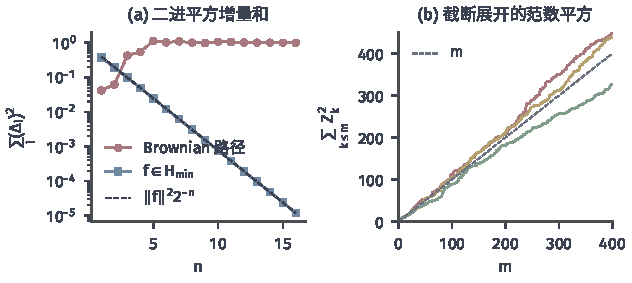
\includegraphics[width=107mm]{figures/03-optimization-evolution-and-signals/02-processes-and-trajectory-evolution/matplotlib/spp-rkhs-vs-path/figure.pdf}
  \caption{Brownian路径与最小值核空间$H_{\min}$的比较。(a)二进平方增量和$Q_n=\sum_i(\Delta_i)^2$随层级$n$的变化（对数纵轴）：红线为一条用$2^{16}$个格点模拟的Brownian路径，蓝线为$f(t)=0.8\sin(\pi t/2)\in H_{\min}$，虚线为上界$\|f\|^2_{H_{\min}}2^{-n}$，其中$\|f\|^2_{H_{\min}}=\int_0^1f'(t)^2\,\mathrm dt=0.08\pi^2\approx0.79$。(b)有限基展开$W^{(m)}$在$H_{\min}$中的范数平方$\sum_{k\le m}Z_k^2$随项数$m$的增长，三条曲线对应三组独立系数，虚线为期望值$m$。随机数均使用固定种子。}
  \label{fig:spp-rkhs-vs-path}
\end{figure}

更一般地，在可分Banach空间上的高斯测度理论中可以证明：协方差的再生核Hilbert空间（在那里称为Cameron--Martin空间）只要是无限维的，其测度就为零。所以对无限维的核，“样本路径属于$H_k$”通常不成立，样本比$H_k$中的典型元素粗糙得多。

\paragraph{两种用途的分工}
$H_k$并没有因此与高斯过程无关。它描述的是：把高斯过程的路径整体平移一个确定函数$h$后，新规律何时与原规律相互绝对连续；答案恰好是$h\in H_k$。第~\ref{chap:continuous-time-stochastic-processes}章研究连续路径的换测度时会用到这一事实的Brownian情形。另一方面，高斯过程回归中，给定有限个观测后的后验均值是$k(\cdot,x_i)$的有限线性组合，因而属于$H_k$；回归、后验及统计保证由卷四的统计推断部分处理。本节的结论是分工：样本路径的正则性由协方差通过增量方差决定，$H_k$刻画的是确定性函数和平移方向，两者不能互相替代。
